\subsection{Review Requirements}
Receiving feedback about the requirements is an important step 
of the management process because it helps ensure the requirements 
are clear and aligned with the scope of the project. 
Helix offers features to help streamline this process.

\subsubsection{Review Mode View}
The Review Mode View is the centre point where users 
can review and comment on requirements. When users open 
a requirement document, they are presented with a hierarchical 
document where they can perform activities related to the review 
process, like adding notes \cite{perforce_2024}.
The image Figure~\ref{fig:review_mode} shows the Review Mode View, with an example of a requirement.

\begin{figure}[htbp]
    \centering
    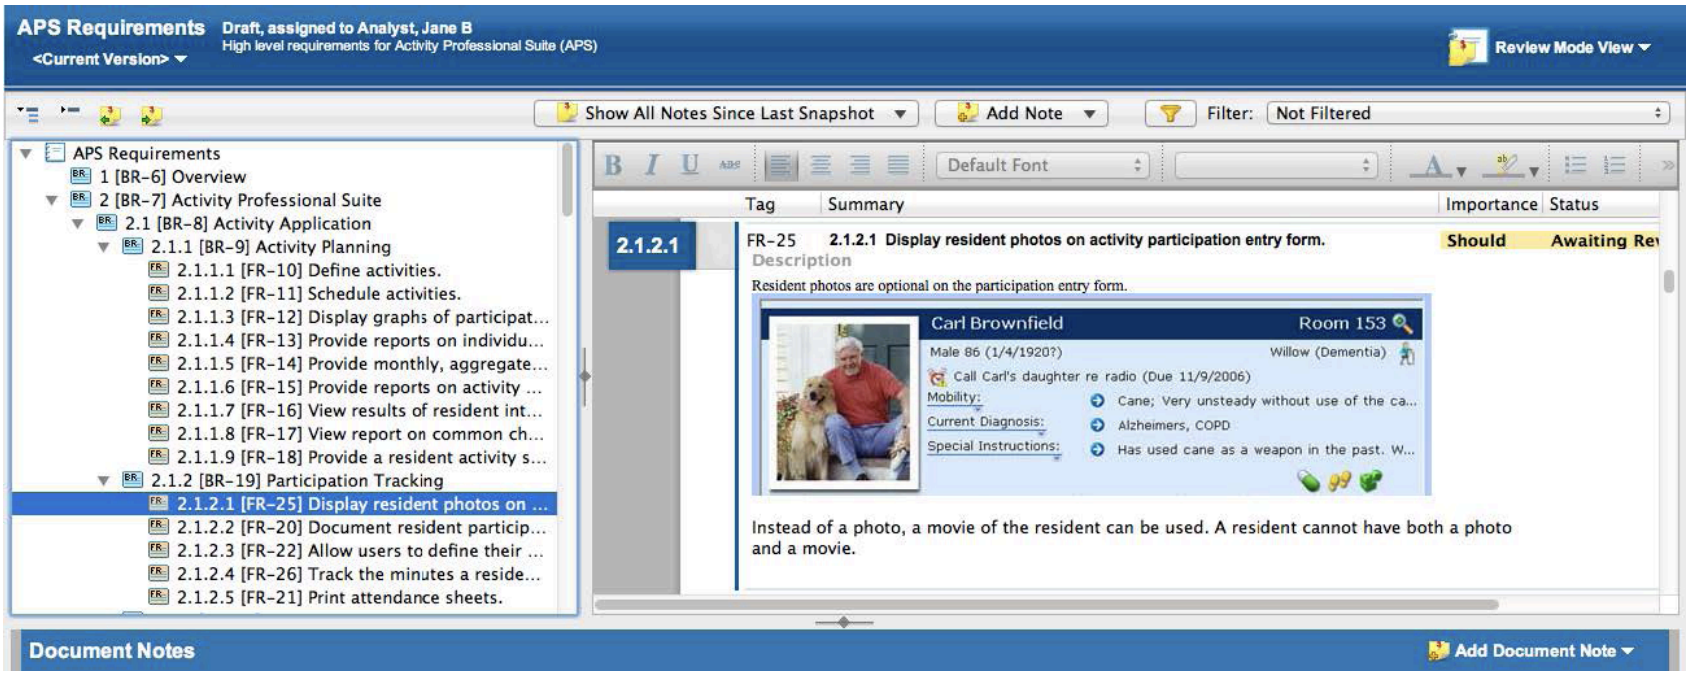
\includegraphics[width=\linewidth]{images/review-mode-view}
    \caption{Helix review mode view.}
    \label{fig:review_mode}
\end{figure}

\subsubsection{Review Feedback}
As part of the process of requirement review, 
Helix gives users the options to add review notes, 
email feedback, or directly edit the requirements.

\paragraph{Review Notes}
Users can add review notes to specific requirements to give 
feedback or ask for changes. The notes are displayed in 
line with the requirements, making it possible to have a 
thread of all feedback given for a requirement \cite{perforce_2024}.
The image Figure~\ref{fig:review_notes} shows an example of a note left in a requirement.

\begin{figure}[htbp]
    \centering
    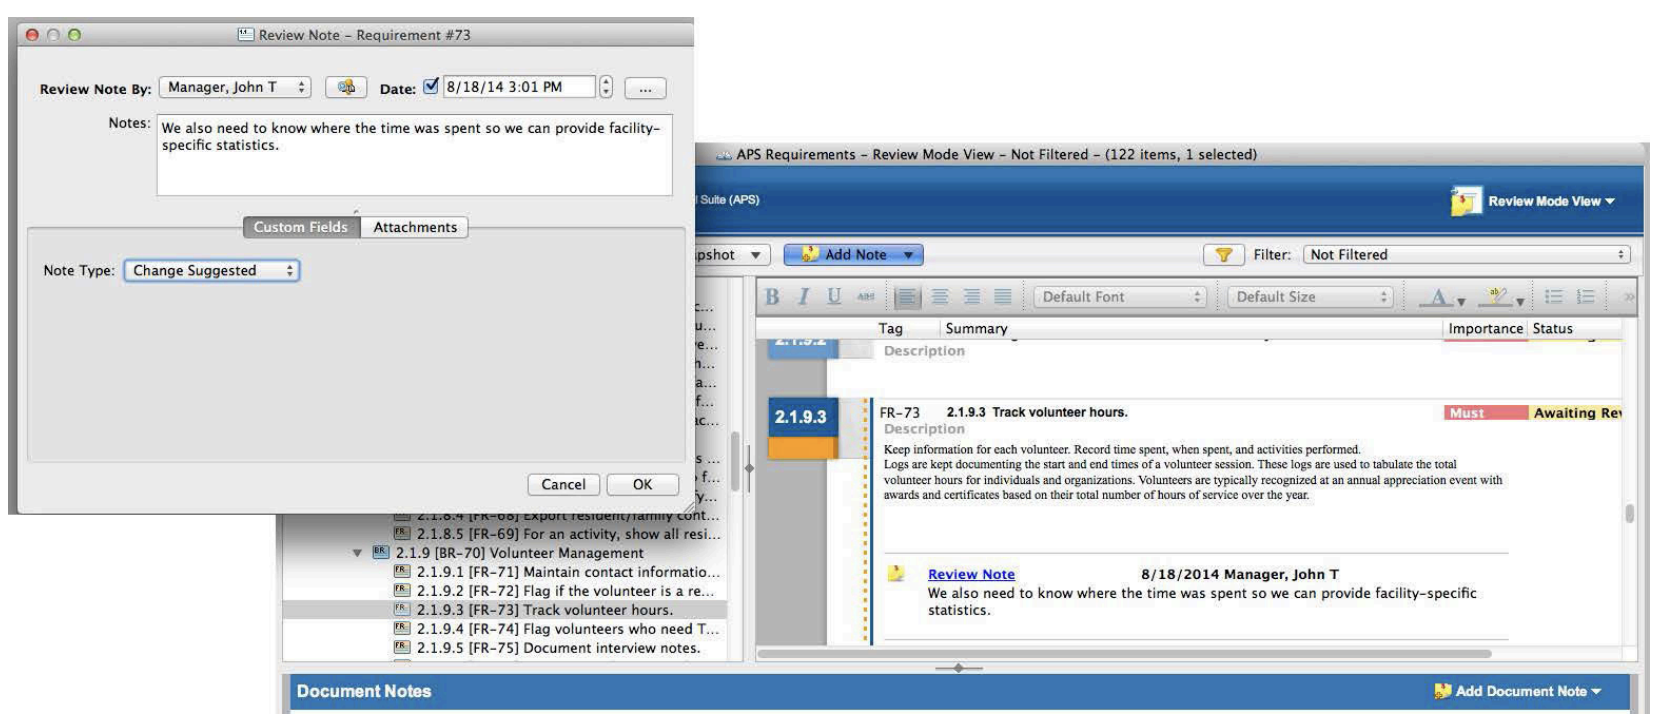
\includegraphics[width=\linewidth]{images/review-notes}
    \caption{Helix review note.}
    \label{fig:review_notes}
\end{figure}


\paragraph{Email Feedback}
Helix makes it possible to email from requirement documents to 
provide feedback. With the enablement of email tracking, 
emails and any subsequent replies are saved with the requirements, 
making it possible to track the full discussion of an item.
The image Figure~\ref{fig:review_email} shows an email panel with an example of feedback in the form of a reply \cite{perforce_2024}.

\begin{figure}[htbp]
    \centering
    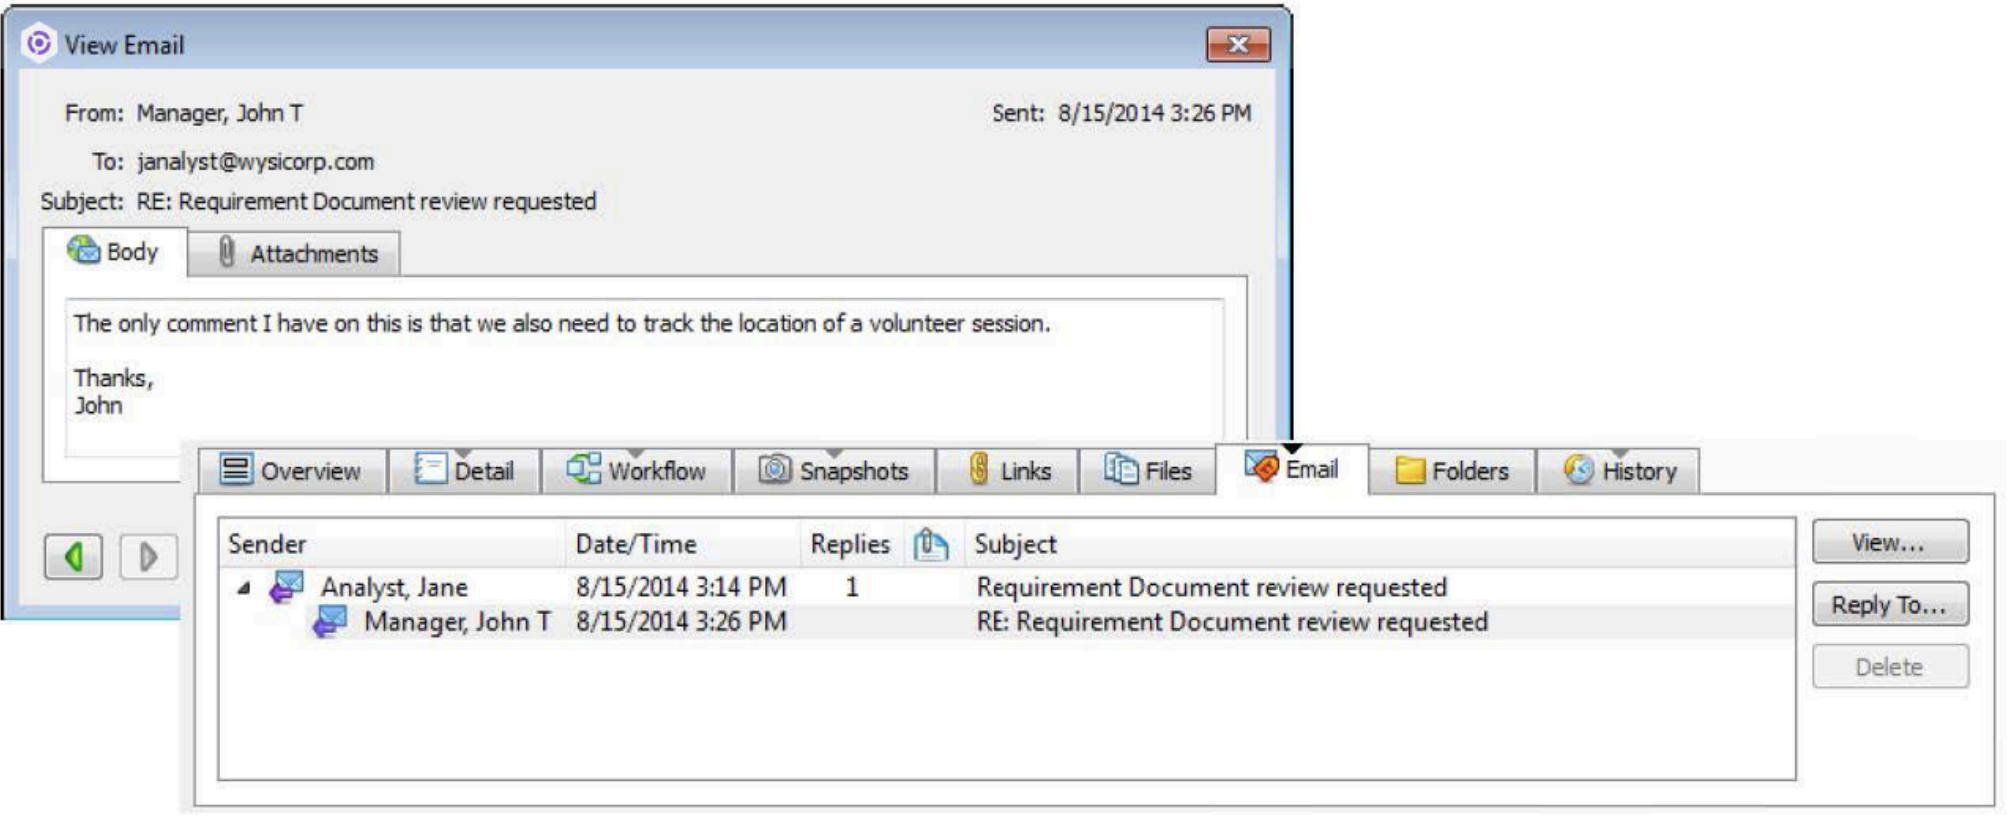
\includegraphics[width=\linewidth]{images/email-feedback}
    \caption{Helix email feedback view.}
    \label{fig:review_email}
\end{figure}

\paragraph{Edit Requirements}
There is also the option to directly change requirements, 
depending on the level of secure permissions. Users can add a 
timestamp with a name to help identify their comments or changes, 
or even apply formatting to the text to make it easier to tell them apart. 
Helix offers the possibility to create a document snapshot to help with requirement changes, 
making it possible to compare old versions with new ones.
The image Figure~\ref{fig:review_edit_feedback} shows a user adding a comment, providing  the timestamp and their name \cite{perforce_2024}.

\begin{figure}[htbp]
    \centering
    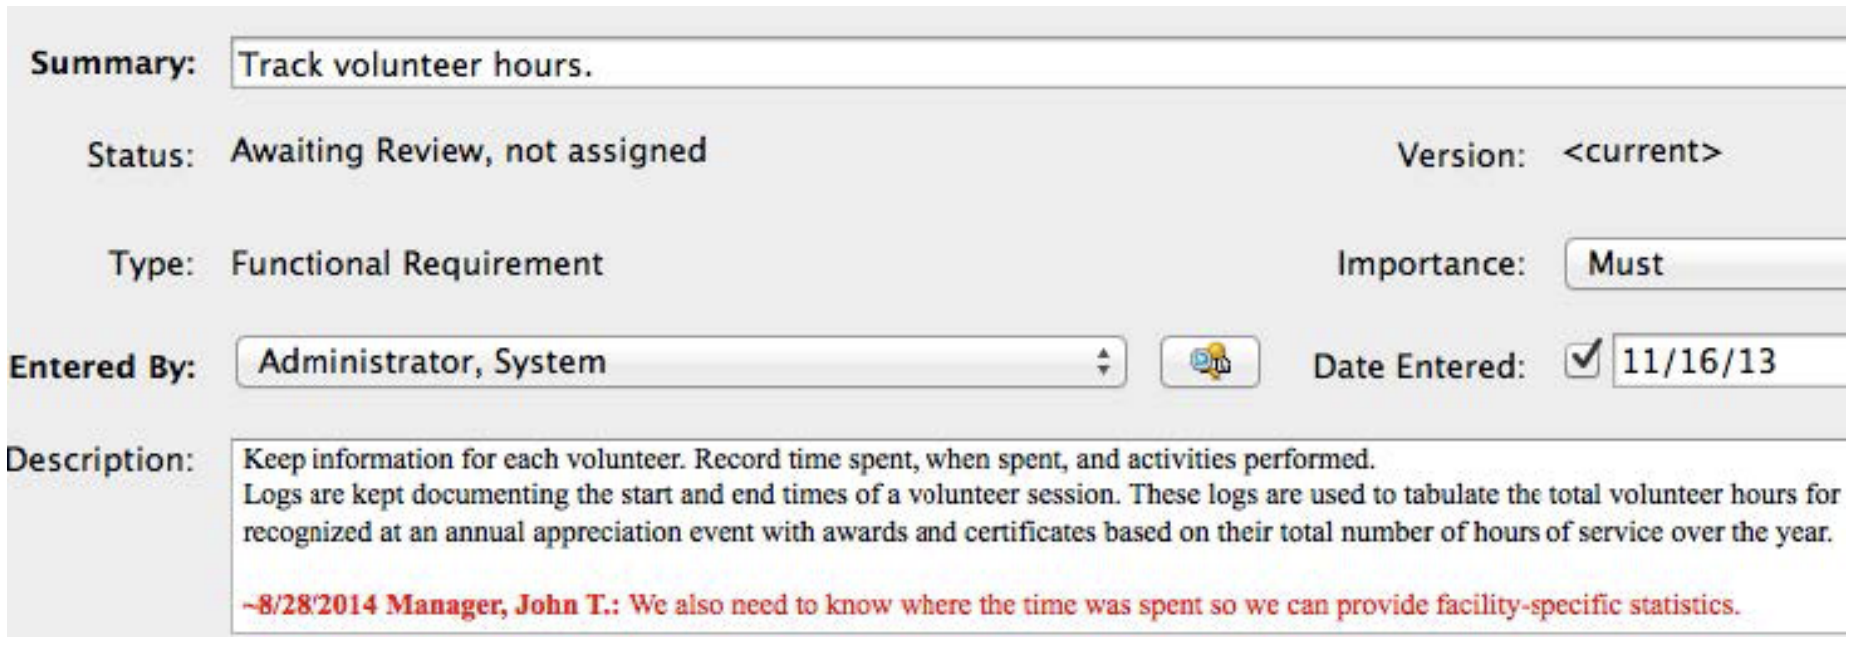
\includegraphics[width=\linewidth]{images/edit-requirements}
    \caption{Helix email feedback view.}
    \label{fig:review_edit_feedback}
\end{figure}